%----------------------------------------------------------------------------------------
%	PACKAGES AND OTHER DOCUMENT CONFIGURATIONS
%----------------------------------------------------------------------------------------
\documentclass[xcolor=dvipsnames]{beamer}

\usepackage[scale=1.24]{beamerposter}
\usepackage{graphicx}
\usepackage{multirow}
\usepackage{array}
\usepackage{tabu}
\usepackage{graphicx} 
\usepackage{booktabs} 
\usetheme{confposter} 

\definecolor{cadet}{rgb}{0.33, 0.41, 0.47}
\definecolor{cadetgrey}{rgb}{0.57, 0.64, 0.69}
\definecolor{bostonunivred}{rgb}{0.9, 0.0, 0.0}
\definecolor{aliceblue}{rgb}{0.94, 0.97, 1.0}

\setbeamercolor{block title}{fg=cadet,bg=white}
\setbeamercolor{block body}{fg=black,bg=white}
\setbeamercolor{block alerted title}{fg=white,bg=cadetgrey}
\setbeamercolor{block alerted body}{fg=black,bg=dblue!10}

%-----------------------------------------------------------

\setlength\parindent{24pt}
\newlength{\sepwid}
\newlength{\onecolwid}
\newlength{\twocolwid}
\newlength{\threecolwid}
\setlength{\paperwidth}{48in} 
\setlength{\paperheight}{36in}
\setlength{\sepwid}{0.024\paperwidth} % Separation width (white space) between columns
\setlength{\onecolwid}{0.22\paperwidth} % Width of one column
\setlength{\twocolwid}{0.464\paperwidth} % Width of two columns
\setlength{\threecolwid}{0.708\paperwidth} % Width of three columns
\setlength{\topmargin}{-0.5in} % Reduce the top margin size

%----------------------------------------------------------------------------------------
%	TITLE SECTION 
%----------------------------------------------------------------------------------------

\title{Predicting Florida Presidential Election Vote Shares} % Poster title

\author{{\huge Sam Yard}}


%----------------------------------------------------------------------------------------

\begin{document}

\addtobeamertemplate{block end}{}{\vspace*{2ex}} % White space under blocks
\addtobeamertemplate{block alerted end}{}{\vspace*{2ex}} % White space under highlighted (alert) blocks

\setlength{\belowcaptionskip}{2ex} % White space under figures
\setlength\belowdisplayshortskip{2ex} % White space under equations

\begin{frame}[t] % The whole poster is enclosed in one beamer frame

\begin{columns}[t] % The whole poster consists of three major columns, the second of which is split into two columns twice - the [t] option aligns each column's content to the top

\begin{column}{\sepwid}\end{column} % Empty spacer column

\begin{column}{\onecolwid} % The first column

%----------------------------------------------------------------------------------------
%	RESEARCH QUESTION AND BACKGROUND
%----------------------------------------------------------------------------------------

\begin{alertblock}{Research Question}
\begin{itemize}
\item[\textcolor{black}{\textbullet}] How do demographic factors, such as population by race, median income, and median housing prices, relate to the 2020 election outcomes in \textbf{Florida} counties?
\item[\textcolor{black}{\textbullet}]  This study investigates the connection between demographic characteristics in Florida counties and their \textbf{political preferences during the 2020 elections}. Florida, known for its diversity and political significance, has historically played a pivotal role in national elections, making it an ideal focal point for this analysis. 
\item[\textcolor{black}{\textbullet}] The research utilizes county-level election results and demographic data from the American Community Survey to provide comprehensive insights into the influence of demographics on election outcomes in Florida.
\end{itemize}
\end{alertblock}

%----------------------------------------------------------------------------------------
%       HYPOTHESES ------------------------------------------------------------------------------------%%%%%%%

\begin{block}{Hypothesis Testing}
\textbf{Linear Model: } \newline
$dem\_votes \sim pop\_poc$ 
\begin{itemize}
\item [\textcolor{black}{\textbullet}] The null hypothesis for the coefficient associated with the variable $pop\_poc$ is: \\
$H_0: \beta_{pop\_poc} = 0$
\item [\textcolor{black}{\textbullet}] Associated Model Results:
\end{itemize}


\begin{tabular}{ |p{5.4cm}|p{5.5cm}|p{5cm}|p{4.5cm}|p{5cm}|}

 \hline
 \multicolumn{5}{|c|}{dem\_votes $\sim$ pop\_poc} \\
 \hline
 & Estimate &Std.Error &t-value & Pr(>|t|)\\
 \hline
 Intercept   & 3.271e+01    &1.569e+00&  20.847 & < 2e-16\\
 \hline
 $pop\_poc$ &  1.995e-05  & 4.266e-06  &4.676 & 1.56e-05\\
 \hline
\end{tabular}

\begin{quote}
\textcolor{white}{\textbullet}This model was employed to investigate the relationship between the Democratic vote share in the 2020 presidential elections, and the percentage of the population that is people of color. $H_0$ suggests no impact of the population of people of color on Democratic vote share. However, the estimated coefficient was found to be statistically significant, providing evidence against $H_0$. The coefficient indicates that an increase in the population of people of color is associated with a corresponding increase in Democratic vote share.
\end{quote}
\end{block}

%------------------------------------------------

\end{column} % End of the first column
\begin{column}{\sepwid}\end{column} % Empty spacer column
\begin{column}{\twocolwid} % Begin a column which is two columns wide (column 2)
\begin{columns}[t,totalwidth=\twocolwid] % Split up the two columns wide column
\begin{column}{\onecolwid}\vspace{-.6in} % The first column within column 2 (column 2.1)

%----------------------------------------------------------------------------------------

\begin{block}{Hypothesis Testing Cont.}

\begin{itemize}
\textbf{Linear Model:} 

$rep\_votes \sim median\_housing\_price$ \\ \newline
\item [\textcolor{black}{\textbullet}] The null hypothesis for the coefficient associated with the variable $median\_housing\_price$ is: \\
$$H_0: \beta_{median\_housing\_price} = 0$$
\item [\textcolor{black}{\textbullet}] Associated Model Results:

\end{itemize}    

\newline
\newline
\begin{tabular}{ |p{5.2cm}|p{5.9cm}|p{5cm}|p{4.2cm}|p{5cm}|}

 \hline
 \multicolumn{5}{|c|}{$rep\_votes \sim median\_housing\_price (mhp)$} \\
 \hline
 & Estimate &Std.Error &t-value & Pr(>|t|)\\
 \hline
 Intercept   & -8.208e+04    &2.710e+04&   -3.029  & 0.00353\\
 \hline
 $mhp$ &   9.406e-01  &1.412e-01   &6.660 & 7.33e-09\\
 \hline
\end{tabular}
\newline

\begin{quote}
\textcolor{white}{\textbullet}This model reveals a significant positive correlation between median housing prices and Republican (0.941, p < 0.00001) votes. These findings suggest that housing affordability, reflected in median prices, may influence political preferences. The interplay of socio-economic factors in shaping electoral dynamics is evident. However, caution is warranted, as correlation does not imply causation. Further research considering additional variables is crucial for a comprehensive understanding of the relationship between housing prices and political preferences in Florida counties.



\end{quote}

\end{block}


\begin{block}{2020 Vote Shares}
\begin{figure}
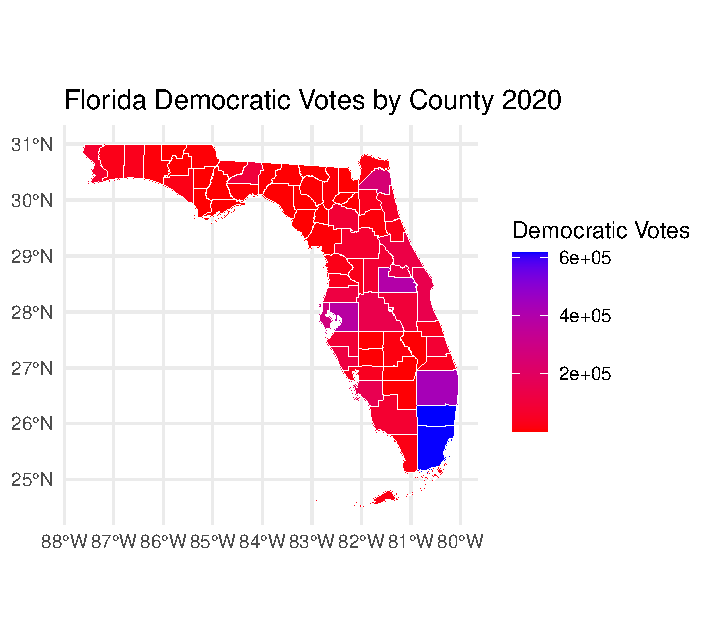
\includegraphics[trim={1.45cm 1cm 1.25cm 1cm},clip,scale=2.7]{dem_votes2020.pdf}
\caption{Florida Vote Share by County 2020}
\end{figure}
\end{block}
\end{column} % End of column 2.1
\begin{column}{\onecolwid}\vspace{-.6in} % The second column within column 2 (column 2.2)

%----------------------------------------------------------------------------------------
%	DEMOGRAPHIC BREAKDOWN
%----------------------------------------------------------------------------------------

\begin{block}{Demographic Impact}

\begin{figure}
\includegraphics[trim={0.2cm 0.2cm 0.5cm 0.8cm},clip,scale=1.9]{race_voteshare.pdf}
\caption{White population vs. 2020 Presidential vote share}
\end{figure}


\begin{tabular}{ |p{5.2cm}|p{5.9cm}|p{5cm}|p{4.2cm}|p{5cm}|}

 \hline
 \multicolumn{5}{|c|}{Average Demographics of Bottom 5 Counties} \\
 \hline
 & Dem Vote Share &White Pop &PoC Pop & House Income\\
 \hline
 Bottom 5 counties   & 14.414\%    &78.54\%&   21.46\% & \$50,012\\
 \hline

\end{tabular}
\newline
\newline
Bottom Five Counties: Holmes, Lafayette, Baker, Dixie, Union

\newline
\begin{tabular}{ |p{5.2cm}|p{5.9cm}|p{5cm}|p{4.2cm}|p{5cm}|}

 \hline
 \multicolumn{5}{|c|}{Average Demographics of Top 5 Counties} \\
 \hline
 & Dem Vote Share &White Pop &PoC Pop & House Income\\
 \hline
 Bottom 5 counties   & 63.86\%    &40.01\% &  59.99\%  & \$53,647\\
 \hline

\end{tabular}
\newline
\newline
Bottom Top Counties: Gadsen, Broward, Leon, Alachua, Orange

\begin{quote}
The top five counties in Florida exhibit a strong Democratic vote share, and reflects a diverse population composition with 59.99\% People of Color. These counties also feature a relatively higher median housing price of \$210,560. In contrast, the bottom five counties have a lower Democratic vote share of 14.41\%, a predominantly White population (78.54\%), and a more affordable median housing price of \$110,500. These findings suggest a correlation between political preferences, racial diversity, and housing affordability in Florida counties. However, a comprehensive understanding would require consideration of additional factors and context.
\end{quote}
\end{block}


%----------------------------------------------------------------------------------------

\end{column} % End of column 2.2

\end{columns} % End of the split of column 2 - any content after this will now take up 2 columns width

\begin{columns}[t,totalwidth=\twocolwid] % Split up the two columns wide column again

\end{columns} % End of the split of column 2

\end{column} % End of the second column

\begin{column}{\sepwid}\end{column} % Empty spacer column

\begin{column}{\onecolwid} % The third column



%----------------------------------------------------------------------------------------
%	RACE HEATMAP
%----------------------------------------------------------------------------------------a
\begin{block}{2020 Population Heatmap by Race}

\begin{figure}
\includegraphics[trim={2.45cm 1.4cm 2.25cm 1.2cm},clip,scale=2.7]{poc_heatmap.pdf}
\caption{Florida Heatmap for Population of People of Color by County}
\end{figure}
\end{block}

%----------------------------------------------------------------------------------------
%	CONCLUSION
%----------------------------------------------------------------------------------------
\begin{block}{Conclusions}\\
\begin{quote}
The models indicate that demographic factors, especially those related to race and the economy, significantly impact Democratic electoral support. Understanding these dynamics is crucial for predicting political preferences in different US regions during large-scale elections.
\end{quote}
\newline
\begin{quote}
For future elections in Florida, socio-economic factors are important considerations. Policymakers and analysts should incorporate these economic dynamics into strategies and forecasts, recognizing the complex nature of political choices. However, it is essential that we consider the entire picture, including various other factors, as the model results do not imply causation.
\end{quote}
\end{block}


%----------------------------------------------------------------------------------------
%	CONTACT
%----------------------------------------------------------------------------------------
\begin{alertblock}{Contact Information}
\begin{enumerate}
    \item [\textcolor{black}{\textbullet}]samyard@bu.edu
\end{enumerate}

\end{alertblock}


\end{column} % End of the third column

\end{columns} % End of all the columns in the poster

\end{frame} % End of the enclosing frame

\end{document}
